%!TEX root = ../thesis.tex

\chapter{Frameworks}
\label{chap:frameworks}

Im Folgenden werden die für den praktischen Teil der Arbeit genutzten Frameworks beschrieben.
Ziel dieses Kapitels ist es, die Auswahl der genannten Frameworks zu begründen und
ihren Funktionsumfang hinsichtlich der Anforderungen des Projekts zu untersuchen.
Des weiteren sollen mögliche Alternativen evaluiert werden.


\section{AngularJS}

Angular ist derzeit eines der populärste Frontend Javascript Frameworks auf dem Markt.
Im nachfolgenden wird der Erfolg des Frameworks anhand eines Interviews mit Robin Böhm erklärt. \cite{Angu68:online}.
Böhm war einer der ersten Entwickler, der Angular 2012 in Deutschland bekannt machte.
``Zu dieser Zeit war jQuery noch die Basis des Webs. jQuery hatte aber nie den Anspruch, ein Framework für Web-Anwendungen zu sein. Der eigentliche Sinn war, die APIs der verschiedenen Browser zu vereinheitlichen.
Man musste sich deshalb immer eine eigene Architektur überlegen. Allerdings fehlte die Erfahrung, wie man große Applikationen im Web schreibt. Das führte natürlich oft zu Chaos und unwartbaren Projekten.''\cite{Angu68:online}
Böhm spricht mit Angular von einem sehr mächtigen Komplettpaket, welches Anwendungsentwicklung im Web auf ein neues Level hebe.
Gründe dafür sind die geringe Lernkurve, simple Template Syntax,
welche auf HTML aufbaut, sowie hohe Wartbarkeit aufgrund einfacher Testbarkeit von einzelnen Appkomponenten.

Wenn Böhm über Angular 2 spricht, spricht er von einem Framework für die Zukunft.
Apps, die zeitnah in Produktion gehen, würde er nach wie vor mit Angular 1 entwickeln,
da Angular2 noch nicht als Release vorliegt und interne Funktionalität auf Browserfeatures basiert,
die teilweise noch nicht in jedem Browser zur Verfügung stehen und daher durch Polyfills implementiert werden müssen.
``Somit wird Angular 2 sein ganzes Potential wohl auch erst in einigen Jahren entfalten können.
Wenn man jedoch erst heute damit anfangen würde, ein Framework für heute zu bauen,
ist es bereits veraltet, wenn es fertig ist.''\cite{Angu68:online}
Zudem sind Style Guides und Best Practise Ansätze für die Entwicklung von Applikationen mit Angular 2
noch in der Entstehung.
Dennoch spricht Böhm zuversichtlich über die Neuentwicklung des Framework.


\subsection{Neuerungen des Framework}

Angular 2 ist die Nachfolgeversion des von Google entwickelten Javascript Framework Angular 1.
Die in 2009 veröffentlichte erste Version fand großen Anklang in der Community
und wurde als Basis für dynamische Single-page-Webanwendung verschiedenster Art und Größe genutzt.
In den seit Release vergangenen Jahren hat sich die Community um das Framework immer weiter vergrößert,
welche zur stetigen Weiterentwicklung und so zu dem Erfolg von Angular1 beigetragen hat.
Das Github Repository der ersten Version hat mittlerweile 1.489 Contributors mit nahezu 7000 gestellten Pull Requests. \cite{ng1-github}

Mit Angular 2 wurden einige Grundkonzepte überarbeitet um in eine komplett neue Richtung gehen zu können.
Ziel von Google ist es, ein komponentenbasiertes leicht zu bedienendes Framework für moderne
Webanwendungen zu schaffen, welches Performanceverbesserungen und transparentere interne Strukturen als die Vorgängerversion aufweisen soll.
Eine Angular 2 Anwendung besteht daher aus einer Vielzahl diverser Komponenten, wodurch es möglich wird
Funktionalität zu kapseln, zu abstrahieren und wieder zu verwenden. Der Fokus hierbei liegt nicht nur auf Wiederverwendbarkeit innerhalb einer Codebasis.
Elemente der Anwendung sollen sowohl für den Browser, als auch für mobile Geräte sowie für native Desktop Clients genutzt werden können.
Angular 2 soll im Vergleich zu seiner Vorgängerversion leichter zu lernen und zu nutzen sein,
sowie eine solide Basis auch für komplexere Webanwendungen bieten. \cite[11-12]{Angular2}


\subsection{Komponenten}

Komponenten sind die Grundbausteine einer jeden Angular 2 Applikation und ersetzen die Direktiven aus Angular 1 nahezu vollständig.
UI und deren Funktionalität wird in Komponenten definiert.
Diese werden in Angular 2 als Typescript Klasse definiert und mit @Component dekoriert.
Der Component Decorator wird mithilfe des ES6 Imports importiert.
Der Selektor definiert den HTML Tag der Komponente, über welchen sie eingefügt und damit instanziiert wird.

Template oder TemplateUrl enthält entweder einen String mit inline Markup in angulars Template Syntax,
oder eine Referenz zu einer zugehörigen HTML Datei, welche das Markup enthält.
Ebenso kann Stylesheet inline oder per Dateireferenz eingebunden sein.
Directives erwartet ein Array von in dieser Komponente zu verwenden weiteren Komponenten.
Ist eine Komponenten als Directive referenziert,
kann ihr Selector im Markup der referenzierenden Komponente eingebunden,
und dadurch ihre Gesamte Funktionalität genutzt werden.
Desweiteren lassen sich durch den Decorator Serviceprovider referenzieren, hierzu jedoch später mehr.

Eine Komponente besteht neben der Decorator Annotation aus einer Klasse.
Daher hat sie einen Klassennamen und mindestens einen impliziten Konstruktor.
Die Klasse wird mit dem ES6 Prefix öffentlich exportiert. Die Sichtbarkeit von Variablen und Funtkionen,
innerhalb der Klasse, kann mithilfe der Prefixe private und public definiert werden.
Dadurch ist es möglich, Funktionalität und Daten in eine Komponente, unsichtbar für deren verwender, zu kapseln.

\vspace{1cm}
\lstinputlisting[language=Java,label=code,caption=Basic Component]{kapitel3/basic-component.ts}
\vspace{1cm}


\subsubsection{Vererbung}

Vererbung, ein Grundkonzept der Objektorientientierung,
wird eingesetzt wenn Verhalten von verschiedenen Objekten zur Wiederverwendung
abstrahiert werden muss. Da Angular 2 Komponenten aus einer Klasse bestehen,
können wir Vererbung Nutzen um Funktionalität von Komponenten zu abstrahieren
um redundanten Code zwischen den Komponenten
zu vermeiden. Logik wird dabei von der Komponente in eine dritte Klasse ausgelagert,
welche mit dem Schlüsselwort extend als
Abstraktionsebene eingebunden wird. \cite{DanWa45:online}


\subsection{Services, Providers und Dependency Injection}

Oftmals bietet es sich an, Funktionalität von Komponenten in Services auszulagern.
Speziell wenn mehrere Komponenten auf die selben Daten,
die womöglich asynchron per HTTP geladen werden müssen, zugreifen.
Services werden ebenfalls als Klassen implementiert, welche mithilfe von \ac{DI}
als Singleton instanziiert und in die Komponenten injiziert werden können.
\ac{DI} ist ein Design Pattern, welches das Framework bereits in der ersten Version implementiert hat.
In Angular 2 wurde \ac{DI} neu entwickel, um die Injizierung von Services in Komponenten zu ermöglichen.

\ac{DI} bringt vielerlei Vorteile mit sich. In der Implementierung einer Angular 2 Komponente wird im
Konstruktor deklariert, welche Abhängigkeiten (Dependencies) für die Komponentenfunktionalität benötigt werden.
Das Framework kümmert sich daraufhin automatisch um die Instanziierung der Objekte.
Die Implementierung einer Komponente wird durch die Verwendung von \ac{DI} sehr flexibel,
da Implementierungen von Services einfach ausgetauscht werden können.
Soll beispielweise die Funktionalität einer Komponente, welche über einen Service dynamisch Daten lädt, getestet werden,
so kann die Implementierung des Services einfach ausgetauscht werden, so dass dieser statische Testdaten liefert,
sollte der Server in der Testumgebung nicht erreichbar sein.
\cite[281]{Angular2}


\vspace{0.3cm}

\begin{figure}[ht]
 \centering
 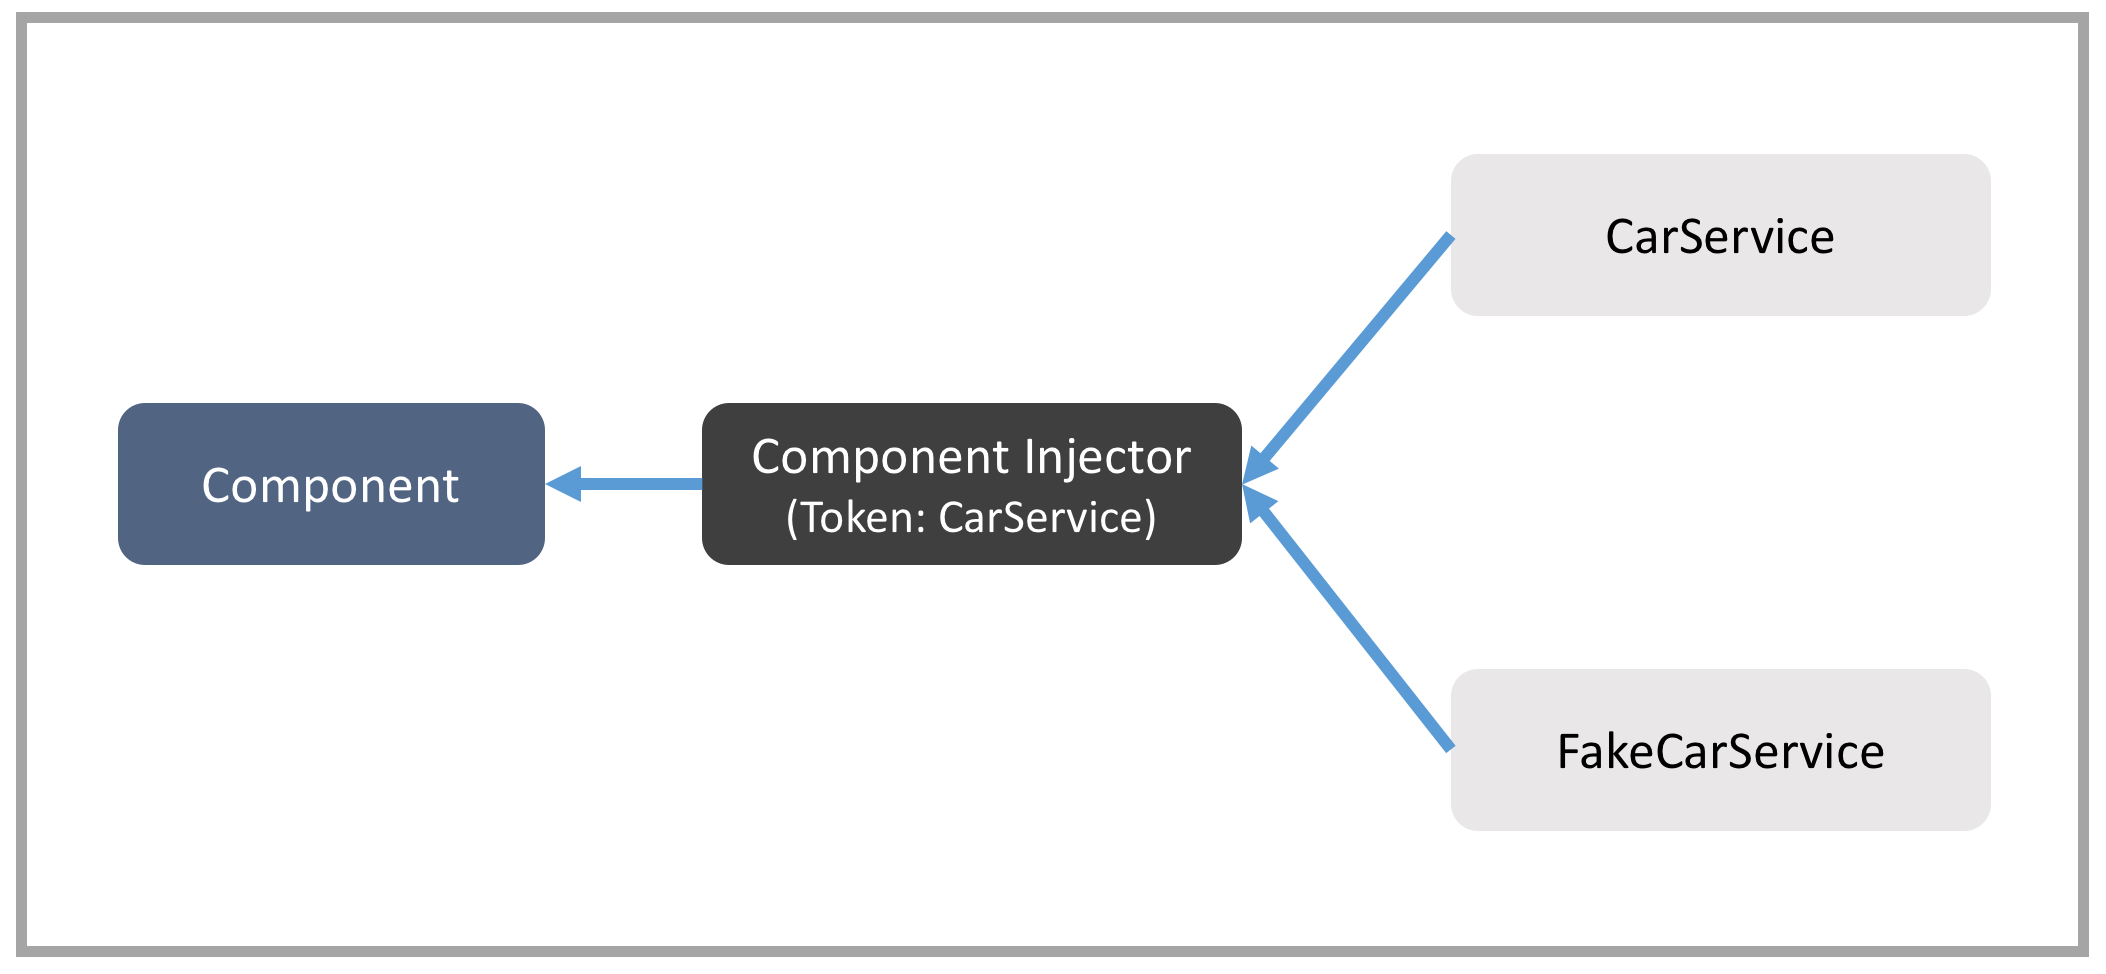
\includegraphics[width=0.8\linewidth]{kapitel3/component-injector.png}
 \caption{Component Injector}\cite[343]{Angular2}
\end{figure}
\vspace{0.3cm}

\ac{DI} wird dabei mithilfe von Providern konfiguriert.
Dies geschieht auf Komponentenebene oder im Root der Applikation.
Wird ein Service über einen Provider im Bootstrap Prozess im Root der Applikation referenziert,
so ist die Instanz des Services in jede Komponente der Applikation injizierbar.
Wird der Provider in der Komponente definiert, so ist die Serviceinstanz in dieser Komponente, sowie in
allen Kindkomponenten verfügbar. Desweiteren lassen sich Provider kombinieren, da diese überschreibbar sind.
Sollte also ein Serviceprovider im Root der Applikation definiert sein, können dennoch weitere Provider in den Komponenten definiert werden.
Jedoch werden demnach auch mehrere Instanzen des Services erzeugt.
Es wäre also möglich, individuelle Singletons für bestimmte Komponentenbäume zu erzeugen. \cite[286]{Angular2}

\vspace{0.2cm}
\lstinputlisting[language=Java,label=code,caption=Provider im Bootstrap Prozess]{kapitel3/provider-example-root.ts}
\vspace{0.2cm}

\vspace{0.2cm}
\lstinputlisting[language=Java,label=code,caption=Provider in einer Komponente]{kapitel3/provider-example.ts}
\vspace{0.2cm}


\subsubsection{Services als Singletons}
\label{Services-als-Singletons}

Wie bereits erwähnt, ermöglichen \ac{DI} Provider Services als Singleton instanziieren zu können.
Dies bringt viele architektonische Vorteile mit sich. Services können auf der einen Seite genutzt werden,
um Funktionalität aus Komponenten zu abstrahieren um in weiteren Komponeten verwendet zu werden,
auf der anderen Seite können sie jedoch auch genutzt werden um Daten multiplen Komponenten zur Verfügung zu stellen.
Das Angular Framework sorgt dafür, dass ein Service nur einmalig instanziiert wird, daher erhalten alle
Komponenten, die den Service injizieren, die selbe Referenz, somit die selbe Instanz und daher die selbe globale Datenbasis.
In einem Userservice könnte beispielweise eine Boolean Variable definiert sein, welche Auskunft darüber gibt,
ob ein User eingeloggt ist, oder nicht. \cite[308]{Angular2}


\subsection{Data Binding}
Das in eine Komponente eingebundene Markup repräsentiert die Viewschicht einer Komponente.
Angular 2 besitzt zur Darstellung von Datenstrukturen eine komplexe, jedoch sehr ausdrucksstarke Template Syntax.
Variablen und Funktionen einer Komponente, können mithilfe von doppelt geschweiften Klammern in die View eingebunden werden.
Auf der Basis von HTML5 können zudem Schleifen und Fallunterscheidungen implementiert werden.
Der Gültigkeitsbereich des Templates bezieht sich, bezüglich Variablen und Funktionen, dabei auf den Kontext der Komponente,
welche das Template in der Component Decoration referenziert. \cite{Templ78:online}

\vspace{1cm}
\lstinputlisting[language=HTML,label=code,caption=Angular 2 Template Syntax]{kapitel3/template-example.html}
\vspace{1cm}

\subsection{Kommunikation}

Da eine Angular 2 Applikation auschlißelich aus Komponenten besteht, müssen diese zwangsweise miteinander
kommunizieren können. Für den Austausch von Daten stehen gibts es verschiedene Ansätze.
Wie bereits in \ref{Services-als-Singletons} erwähnt, werden Services im Normalfall als Singleton
instanziiert und in Komponenten mittels \ac{DI} injiziert. Öffentliche Servicefunktionen können hierbei für den
Austausch von Daten genutzt werden. Über den synchronen Zugriff auf Variablen hinaus,
können Events in Komponenten oder Services definiert, und von derer ebenfalls aboniert werden,
um asynchrone Kommunikation applikationsintern zu ermöglichen.

Die Auslagerung von Funktionalität in Services macht jedoch nur dann wirlich Sin,
wenn diese auch als Singleton existieren kann. Komponenten sind im vergleich zu Services keine Singletons,
da sie mit jeder Verwendung in der Applikation neu instanziiert werden.
Variablen und Funktionen, eingebundener Komponenten, können durch die Annotationen Input und Output
direkt über den HTML Component Tag angesprochen werden. Im Normalfall werden bei der Instanziierung von Kindkomponenten
relevante Daten über den Input Tag übergeben und über den Output Kanal werden Event Emitter aboniert. \cite{Angul94:online}

Spricht man speziell von Kindkomponenten und nicht von Nachbarkomponenten,
kann mithilfer der Annotation ViewChild auf den öffentlichen Kontext der Kindkomponente zugegriffen werden.
Die Kommunikation geschieht in diesem Fall nicht über die beiden View Layer der Komponenten,
sondern direkt von der Elternkomponente zu ihrer Kindinstanz. \cite{ViewC61:online}

\subsection{Performance}

\subsubsection{Serverside Rendering}

\subsubsection{Change Detection}

Starten wir eine Angular2 Applikation, wird uns als Nutzer nach dem anfänglichen Laden der Seite eine View gerendert.
Eine interne Datenstruktur wird dabei per Templating auf eine Viewstruktur, den DOM, abgebildet und uns als Nutzer somit mittels Text,
Formularen, Buttons, Bildern etc. visuell aufbereitet wird.
Gibt es nun Änderungen in der Datenstruktur zur Laufzeit, muss die View dementsprechend aktualisiert werden.
Zugriffe auf den DOM sind ressourcenintensiv, daher sollten DOM Manipulationen nicht inflationär stattfinden.
Datenänderungen können entwerder durch User Events, XMLHttpRequests oder Timer (setTimeout(), setInterval()) ausgelöst werden.
Alle dies geschieht asynchron. Wir können also davon ausgehen, dass sobald eine asynchrone Aktivität innerhalb einer Komponente auftritt,
sich womöglich Daten geändert haben und die View aktualisiert werden muss.
\cite{changedetection-explained}

\subsubsection{NgZone}

Zones sind ein internes Feature der Programmiersprache Dart. Da Dart jedoch zu JavaScript compiliert werden kann,
können Zones ebenfalls in JavaScript genutzt werden. Daher ist zone.js als Portierung für JavScript entstanden, welche in Angular2 genutzt wird.
Zones sind Ausführungskontexte, für die Observation asynchroner Operationen.
Asynchrone Funktionen werden mittels Monkey Patching überwacht und lösenen in den entsprechenden Ausführungskontexten diverse Events aus.
NgZone ist ein Fork von zone.js, welcher die Basisfunktionalität um zusätzliche Events erweitert.
Change Detection relevant ist dabei das event onTurnDone().
\cite{changedetection-explained}

\vspace{0.5cm}
\textbf{``onTurnDone() - Notifies subscribers immediately after Angular’s zone is done processing the current turn and any micro tasks scheduled from that turn.''}
\cite{ZONESINANGULAR2}
\vspace{0.5cm}

Sobald das onTurnDone() Event ausgelöst wird, löst NgZone wiederum eine tick() Event aus, welches Schlussendlich die Change Detection startet.
Jede Angular2 Komponente besitzt seinen eigenen Change Detector. Da wir bereits wissen, dass eine Angular2 Applikation aus einem Komponentenbaum besteht,
können wir davon ausgehen, dass sie ebenfalls aus einem Baum von Change Detectoren besteht.
Change Detection wird innerhalb dieses Baumes als unidirektionaler Datenfluss von Oben nach Unten, beginnend mit dem Rootknoten, ausgeführt.

Obwohl jede Komponente bei einem tick() nach Änderungen prüft, ist Angular2 unglaublich schnell. Es können mehrere 100.000 Checks in wenigen Millisekunden durchgeführt werden,
da jede Komponenten ihren eigenen Change Detector besitzt und es nicht die eine große Instanz gibt, die alle Komponenten zeitgleich observieren muss.
Dies wird erreicht indem Angular zur Laufzeit individuelle Change Detector Klassen für jede Komponente, entsprechend dem Datenmodell der Komponente erzeugt.
Dieser Code kann von Virtuellen Maschinen optimiert und daher vergleichsweise schnell ausgeführt werden.

\vspace{1cm}

\begin{figure}[ht]
 \centering
 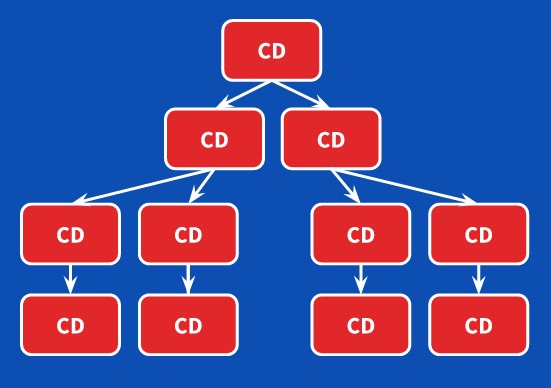
\includegraphics[width=0.7\linewidth]{kapitel3/cd-tree.jpg}
 \caption{Change Detection Flow}\cite{changedetection-explained}
\end{figure}


\section{Ionic}
\subsection{Allgemein}
\subsection{Komponenten verwenden}
\subsection{Deployment}

\section{Electron}
\subsection{Allgemein}
